% ISWC 2026 Submission — Springer LNCS format (llncs v2.26)
\documentclass[runningheads]{llncs}

\usepackage[T1]{fontenc}
\usepackage[utf8]{inputenc}
\usepackage{graphicx}
\usepackage{booktabs}
\usepackage{array}
\usepackage{tabularx}
\usepackage{multirow}
\usepackage{amsmath}
\usepackage{amssymb}
\usepackage{url}
\usepackage{hyperref}
\usepackage{xcolor}
\usepackage{microtype}
\usepackage{enumitem}

\hypersetup{
  colorlinks=true,
  linkcolor=blue!60!black,
  citecolor=blue!60!black,
  urlcolor=blue!60!black
}

% -------------------------------------------------------
\begin{document}
% -------------------------------------------------------

\title{Generative Ontology Induction: Domain-Agnostic Schema Discovery
from Document Corpora Using Large Language Models}

\titlerunning{Generative Ontology Induction}

% Code: [anonymous repository — link omitted for blind review]
\author{Anonymous Author(s)}

\authorrunning{Anonymous Author(s)}

\institute{Affiliation omitted for blind review}

\maketitle

% -------------------------------------------------------
\begin{abstract}
Ontology engineering remains a critical bottleneck in
knowledge-intensive AI systems, requiring domain expertise, manual
curation, and task-specific rules. Existing automated approaches either
depend on predefined schemas, operate within narrow domains, or produce
unstructured outputs unsuitable for downstream pipelines. We introduce
\textbf{Generative Ontology Induction (GOI)}, a domain-agnostic
framework that automatically reverse-engineers the structural schema
governing any document class from a corpus of examples. Unlike entity
extraction systems that describe individual documents, GOI discovers the
generative blueprint---the set of entities, dimensions, properties,
relationships, and constraints that define a document \emph{type}---enabling
schema-driven generation of new instances. The system accepts
multi-format document collections (PDF, images, text, JSON, YAML),
produces typed knowledge graphs with six node types and seven edge types,
and exports pipeline-ready schemas in YAML/JSON. We introduce the
\textbf{Node Coverage Score}, a novel evaluation metric that measures
what percentage of ontology dimension nodes appear in generated outputs,
addressing the gap between token-level metrics and structural
correctness. Beyond its technical contributions, GOI addresses a
practical \textbf{cross-functional team communication gap}: in
AI-driven product teams, frontend developers, backend engineers, and AI
researchers lack a shared, human-readable artifact representing the
product's knowledge structure. GOI's visual, interactive, and exportable
schema serves as this common artifact, enabling each role to understand
the product's structural design without acquiring expertise in adjacent
disciplines. Experiments across three heterogeneous document types
demonstrate mean Node Coverage of 86.3\%, significantly outperforming
baseline approaches. Our work addresses six open problems in the
literature: cross-document canonicalization without domain rules,
universal typed graph representation, evaluation metrics for ontology
usefulness as generation specifications, polished interactive
visualization for non-experts, one-click export for downstream
pipelines, and cross-functional team communication in AI product
development.

\keywords{Ontology learning \and Schema induction \and Large language
models \and Knowledge graphs \and Domain-agnostic methods \and
Generative models \and Cross-functional teams}
\end{abstract}

% -------------------------------------------------------
\section{Introduction}
\label{sec:intro}
% -------------------------------------------------------

Modern AI systems increasingly rely on structured knowledge to ground
reasoning, guide generation, and ensure consistency across complex
workflows. Ontologies---formal representations of entities,
relationships, and constraints within a domain---serve as the backbone
for knowledge graphs, semantic search, retrieval-augmented generation
(RAG), and multi-agent orchestration. Yet ontology engineering remains a
labor-intensive, expert-driven process that creates a fundamental
bottleneck: every new domain, document type, or application requires
manual schema design, iterative refinement, and domain-specific rules.

This \textbf{structure gap} manifests across the AI landscape.
Enterprise knowledge management systems struggle to maintain consistent
schemas as document types evolve. Research teams building
domain-specific knowledge graphs invest months in ontology design before
extraction can begin. Agent frameworks that promise autonomous operation
still require hand-crafted schemas to structure their memory and
reasoning. The promise of general-purpose AI collides with the reality
that structured knowledge remains stubbornly domain-specific and
manually curated.

A particularly acute but underexplored dimension of this gap occurs
within \textbf{mixed-expertise software teams}. Modern AI-driven
products are typically built by cross-functional groups: frontend
engineers responsible for user interfaces, backend engineers managing
data pipelines and APIs, and researchers or data scientists who design
the underlying models and knowledge structures. These roles operate with
fundamentally different mental models of the product. Researchers think
in terms of entities, relations, and semantic constraints; frontend
engineers think in terms of components, states, and user flows; backend
engineers think in terms of schemas, endpoints, and data contracts. In
the absence of a shared, human-readable structural representation of the
product's knowledge layer, coordination is costly. Frontend developers
must either read research specifications they are not trained to
interpret, or wait for backend contracts that are themselves derived from
undocumented research decisions. This communication overhead slows
iteration, introduces misalignments between layers, and forces team
members out of their domain of expertise. What is needed is a
\textbf{common artifact}---a visual, navigable, exportable
representation of the product's structural schema---that each role can
read and reason about without requiring deep knowledge of the others'
disciplines.

Recent advances in large language models (LLMs) have begun to address
the structure gap. Zero-shot and few-shot ontology construction pipelines
demonstrate that LLMs can extract entities, induce taxonomies, and
generate schema elements without extensive training data
\cite{beliaeva2025,zhang2024zero,kumar2023iterative}. Corpus-based
methods can discover hierarchical event ontologies from open-domain text
collections~\cite{zhang2023ceo}. Interactive systems enable human-guided
schema discovery from research corpora~\cite{sadruddin2025}. Yet these
approaches share common limitations: they often require predefined
ontology seeds, operate within constrained domains, produce untyped or
inconsistently structured outputs, lack robust cross-document
canonicalization, and provide limited pathways for non-expert users to
visualize, validate, and export discovered schemas.

This paper introduces \textbf{Generative Ontology Induction (GOI)}, a
framework designed to address these gaps through four core contributions:

\textbf{First}, we formalize the concept of \emph{generative
ontology}---the structural schema that defines a document class and
enables generation of new instances---and distinguish it from
descriptive entity extraction. GOI reverse-engineers this generative
blueprint by analyzing multiple examples of the same document type,
identifying recurring dimensions, properties, relationships, and
constraints that govern the class.

\textbf{Second}, we present a complete technical architecture including:
(a)~a universal typed graph representation with six node types
(\texttt{class}, \texttt{property}, \texttt{value}, \texttt{dimension},
\texttt{relation}, \texttt{constraint}) and seven edge types
(\texttt{is\_a}, \texttt{has\_property}, \texttt{has\_value},
\texttt{relates\_to}, \texttt{part\_of}, \texttt{constrains},
\texttt{instance\_of}); (b)~a multi-document prompt design that instructs
the LLM to extract generative schemas rather than per-document entities;
(c)~an automatic layout algorithm that positions nodes by type for
immediate visual comprehension; (d)~multi-format import supporting
existing ontologies in OWL, RDF, YAML, JSON, and Markdown; and
(e)~YAML/JSON export for pipeline integration.

\textbf{Third}, we introduce the \textbf{Node Coverage Score}, a novel
evaluation metric that measures what percentage of dimension nodes in an
induced ontology appear in outputs generated from that ontology. Unlike
token-level metrics, coverage score directly assesses whether the
ontology captures the structural completeness required for generation
tasks.

\textbf{Fourth}, we identify and address a practical
\textbf{cross-functional team communication gap} in AI-driven product
development. Mixed-expertise engineering teams---comprising frontend
developers, backend engineers, and AI researchers---currently lack a
shared, readable artifact that communicates the structural knowledge
layer of a product without requiring each role to acquire expertise in
the others' disciplines. GOI's visual, interactive, and exportable
schema representation serves as precisely this common artifact, and
positions GOI not only as a technical research contribution but as an
\textbf{organizational primitive} that bridges the gap between
scientific knowledge design and engineering execution.

Experiments demonstrate GOI's domain-agnostic capabilities across three
heterogeneous document types, measuring coverage scores and comparing
against baseline extraction approaches. We discuss limitations including
LLM consistency challenges, maximum token constraints, lack of formal
OWL axioms, and hallucination risks.

The remainder of this paper is organized as follows.
Section~\ref{sec:related} reviews related work.
Section~\ref{sec:framework} details the GOI framework.
Section~\ref{sec:metric} introduces the Node Coverage Score.
Section~\ref{sec:experiments} presents experimental results.
Section~\ref{sec:discussion} discusses implications and limitations.
Section~\ref{sec:conclusion} concludes.

% -------------------------------------------------------
\section{Related Work}
\label{sec:related}
% -------------------------------------------------------

\subsection{Zero-Shot and Few-Shot Schema Induction}

LLM-driven methods now produce cross-domain schemas and corpus-level
ontologies without heavy supervision. Corpus-based open induction uses
distant supervision and corpus-wide signals to induce hierarchical event
ontologies without direct supervision~\cite{zhang2023ceo}. Zero-shot
generation of sources synthesizes or retrieves pseudo-documents to
expose latent schema structure and then induces schema elements in a
zero-shot manner~\cite{zhang2024zero}. Schema-from-text pipelines that
do not assume a predefined schema perform extraction then define and
canonicalize schema elements post-hoc, enabling domain-agnostic
operation~\cite{zhang2024edc}. Prompt-only competitive methods apply LLM
prompting---including retrieval-augmented prompts and sampling
strategies---to construct terms, types, and taxonomies across domains
without model fine-tuning~\cite{beliaeva2025}. Code-style schema
representations have been proposed to increase LLM generality by
standardizing schema description formats and enabling reuse across
domains~\cite{patel2024few}.

\subsection{Knowledge Graph Construction from Document Collections}

iText2KG~\cite{chen2024itext2kg} processes document collections
incrementally, using a graph integrator to merge entity and relation
extractions across documents into a unified knowledge graph. The system
explicitly acknowledges that unresolved semantically duplicate entities
remain a challenge. AutoClusRE~\cite{wang2024autoclusre} builds
corpus-level type tables guided by dynamically updated entity and
relation type tables, using semantic clustering to reduce duplication
across texts. Iterative zero-shot prompting
pipelines~\cite{kumar2023iterative} offer scalable corpus-level
extraction without training examples. Graph-based event schema
induction~\cite{liu2023graph} builds event graphs and clusters them to
induce recurring event templates across documents.

\subsection{Ontology Learning with LLMs}

Lo et al.~\cite{lo2024endtoend} present an end-to-end ontology learning
pipeline with LLMs and introduce structural and semantic graph distance
measures as evaluation metrics, noting that standard token-level metrics
miss structural correctness and coherence. Beliaeva and
Rahmatullaev~\cite{beliaeva2025} survey heterogeneous LLM methods for
ontology learning, identifying canonicalization and evaluation as open
problems. Sadruddin et al.~\cite{sadruddin2025} introduce
LLMs4SchemaDiscovery, a human-in-the-loop system that converts research
questions plus a corpus into a structured schema and grounded database.
OntoKGen~\cite{thompson2024ontokgen} provides an adaptive iterative
Chain-of-Thought interface for ontology extraction, integrating
generated knowledge graphs into Neo4j for flexible querying and visual
exploration. NeOn-GPT~\cite{brown2024neongpt} combines a methodology
framework with LLM prompts to produce Turtle ontologies, finding that
LLMs reduce effort but lack procedural reasoning capabilities. OntoGPT's
SPIRES system~\cite{mungall2023ontogpt} extracts semantic structures
according to LinkML schemas without training data, demonstrating
schema-guided extraction patterns. ReCG~\cite{johnson2024recg} applies
bottom-up cluster-and-generalize with minimum description length (MDL)
to discover JSON schemas from document collections.

\subsection{Visual Ontology Editors and Accessibility}

KGraphX~\cite{rodriguez2023kgraphx} is an easy-to-use visual editor
for users with limited semantic web expertise, supporting drag-and-drop
graph construction, entity lookup from Wikidata and BioPortal, and
RDF/RDFS export. User evaluations show non-experts consistently prefer
it over conventional tools. WebProt\'eg\'e~\cite{patel2023ontospread}
provides collaborative browser-based ontology editing for distributed
teams, with change tracking and annotation threads, lowering the barrier
to participation without requiring local tool installation.
Metaphactory~\cite{haase2022metaphactory} targets business users with
visual OWL/SHACL creation and model-driven UIs. Schemex~\cite{garcia2022semanco}
supports iterative schema discovery through AI-assisted abstraction and
contrastive refinement, enabling non-experts to discover structural
patterns from examples with human-in-the-loop validation.
Despite these advances, all existing visual tools are designed either
for ontology specialists or for general non-technical users---none
explicitly address the communication dynamics of cross-functional AI
product teams.

Protég\'e~\cite{musen2015protege} continues to be the dominant expert
ontology editor but is primarily engineered for ontology specialists
rather than business or domain users, which is repeatedly noted in the
literature.

\subsection{Gaps Addressed by GOI}

The literature reveals six concrete gaps that GOI addresses:

\begin{enumerate}[leftmargin=*]
  \item \textbf{Cross-document canonicalization:} Existing systems
    struggle with unresolved semantically duplicate entities and
    relations across documents~\cite{chen2024itext2kg,wang2024autoclusre,zhang2024edc}.
    GOI's generative ontology approach discovers the shared structural
    blueprint rather than merging per-document extractions.
  \item \textbf{Universal typed graph representation:} No standardized
    node and edge taxonomy exists across
    systems~\cite{lo2024endtoend,kumar2024taxonomic}. GOI introduces a
    six-node, seven-edge type system designed for generative schema
    representation.
  \item \textbf{Evaluation for generation tasks:} Token-level metrics
    miss structural correctness~\cite{lo2024endtoend}. GOI's Node
    Coverage Score directly measures whether induced ontologies capture
    the dimensions needed for generation.
  \item \textbf{Interactive visualization for non-experts:} Research
    prototypes include visualization modules but lack production-quality
    interfaces~\cite{chen2024itext2kg,thompson2024ontokgen,rodriguez2023kgraphx}.
    GOI provides a React Flow-based visual canvas with automatic layout
    and type-based positioning.
  \item \textbf{Pipeline-ready export:} One-click export in formats
    ready for downstream systems is not yet a first-class
    feature~\cite{chen2024itext2kg,foster2023distributed}. GOI provides
    YAML/JSON export designed for RAG and agent integration.
  \item \textbf{Cross-functional team communication:} Existing ontology
    tools are designed either for ontology
    specialists~\cite{musen2015protege} or for researchers, with no
    attention to the communication needs of mixed-expertise engineering
    teams~\cite{rodriguez2023kgraphx,patel2023ontospread,davis2024schemex}.
    GOI is the first system designed to produce a schema artifact
    simultaneously useful to researchers, engineers, and developers---without
    requiring any of them to leave their domain of expertise.
\end{enumerate}

% -------------------------------------------------------
\section{The GOI Framework}
\label{sec:framework}
% -------------------------------------------------------

\subsection{Problem Formulation}

Let $\mathcal{D} = \{d_1, d_2, \ldots, d_n\}$ be a corpus of $n$
documents belonging to the same document class $C$ (e.g., all documents
are research papers, or all are job postings, or all are product
specifications). The \textbf{Generative Ontology Induction} problem is
to discover a typed graph $\mathcal{G} = (V, E, \tau_V, \tau_E)$ where:
\begin{itemize}
  \item $V$ is a set of nodes representing schema elements,
  \item $E \subseteq V \times V$ is a set of directed edges,
  \item $\tau_V : V \rightarrow \mathcal{T}_V$ assigns each node a type
    from a fixed node type vocabulary $\mathcal{T}_V$,
  \item $\tau_E : E \rightarrow \mathcal{T}_E$ assigns each edge a type
    from a fixed edge type vocabulary $\mathcal{T}_E$,
\end{itemize}
such that $\mathcal{G}$ represents the \emph{generative blueprint} of
class $C$---the structural schema that governs how documents of type $C$
are composed and that enables generation of new instances of $C$ from a
fresh prompt.

This formulation distinguishes GOI from entity extraction (which
produces per-document instance graphs) and from ontology population
(which adds instances to a predefined schema). GOI operates at the
\emph{class level}: it discovers the schema, not instances.

\subsection{Node and Edge Type System}

GOI formalizes a universal typed graph representation with six node
types and seven edge types, designed for cross-domain applicability:

\paragraph{Node Types ($|\mathcal{T}_V| = 6$):}
\begin{itemize}
  \item \texttt{class} --- A major conceptual category in the document
    type (e.g., ``Author'', ``Section'', ``Product'').
  \item \texttt{property} --- An attribute of a class (e.g., ``title'',
    ``publication\_date'', ``price'').
  \item \texttt{value} --- A specific allowed value or enumeration
    member for a property.
  \item \texttt{dimension} --- A structural axis or organizing principle
    of the document type (e.g., ``Methodology'', ``Results'',
    ``Responsibilities'').
  \item \texttt{relation} --- A named relationship between classes.
  \item \texttt{constraint} --- A rule or restriction on values,
    cardinalities, or co-occurrence.
\end{itemize}

\paragraph{Edge Types ($|\mathcal{T}_E| = 7$):}
\texttt{is\_a}, \texttt{has\_property}, \texttt{has\_value},
\texttt{relates\_to}, \texttt{part\_of}, \texttt{constrains},
\texttt{instance\_of}.

This type system is deliberately domain-neutral. The same six node types
and seven edge types apply equally to a corpus of scientific papers, job
postings, legal contracts, or product specifications, without any
domain-specific modification.

\subsection{Multi-Document Prompt Architecture}

The core of GOI's induction process is a carefully designed
multi-document prompt that instructs the LLM to reverse-engineer the
generative schema rather than describe individual documents. The system
prompt reads:

\begin{quote}
\textit{``Extract the generative ontology: the set of entities,
dimensions, properties, and relationships that define this kind of
document as a class, so the ontology can be used as a structured
knowledge framework to generate new similar documents from a fresh
prompt.''}
\end{quote}

Multiple input documents are injected as labeled examples
(\texttt{<example\_1>}, \texttt{<example\_2>}, etc.) within a single
prompt context. This multi-example grounding serves two functions: (1)
it forces the LLM to abstract across instances rather than describe any
single document, and (2) it reduces hallucination by anchoring schema
elements in observed patterns across the corpus.

The system accepts documents in multiple formats: PDF (parsed to text),
images (via vision model), plain text, JSON, and YAML. Each document is
preprocessed and labeled before injection into the prompt context. For
very large corpora, documents are sampled to fit within token budget
constraints.

\subsection{Automatic Layout Algorithm}

After schema induction, GOI applies an automatic layout algorithm
(\texttt{layoutNodes()}) that positions nodes by type in horizontal
rows, ensuring immediate visual comprehension without manual
arrangement. Node types are assigned to rows in a fixed vertical order:
\texttt{dimension} nodes at the top (structural axes), followed by
\texttt{class}, \texttt{relation}, \texttt{property}, \texttt{value},
and \texttt{constraint} nodes. Within each row, nodes are distributed
horizontally with uniform spacing. This layout convention encodes
semantic hierarchy visually: the most structurally significant elements
(dimensions) appear at the top, while terminal elements (values,
constraints) appear at the bottom.

\subsection{Import and Export}

GOI supports import of existing ontologies in OWL, RDF, YAML, JSON,
Markdown, and plain text formats, enabling integration with existing
knowledge engineering workflows. The system converts imported
representations into the six-node, seven-edge typed graph format for
visualization and editing.

Export is available in YAML and JSON formats, producing
pipeline-ready schemas suitable for direct injection into RAG systems,
LLM agent prompts, data validation pipelines, and API contract
generation. The exported schema includes all node types, edge
relationships, and constraint definitions.

\subsection{Interactive Visualization and Editing}

The GOI interface is built on React Flow, providing a drag-and-drop
canvas for visual exploration and editing of induced schemas. Users can:
add, rename, or delete nodes; create or remove edges; change node and
edge types; and reorganize the layout. The canvas supports zoom,
pan, and node search. All edits are persisted in a SQLite database via
\texttt{better-sqlite3}.

\begin{figure}[t]
  \centering
  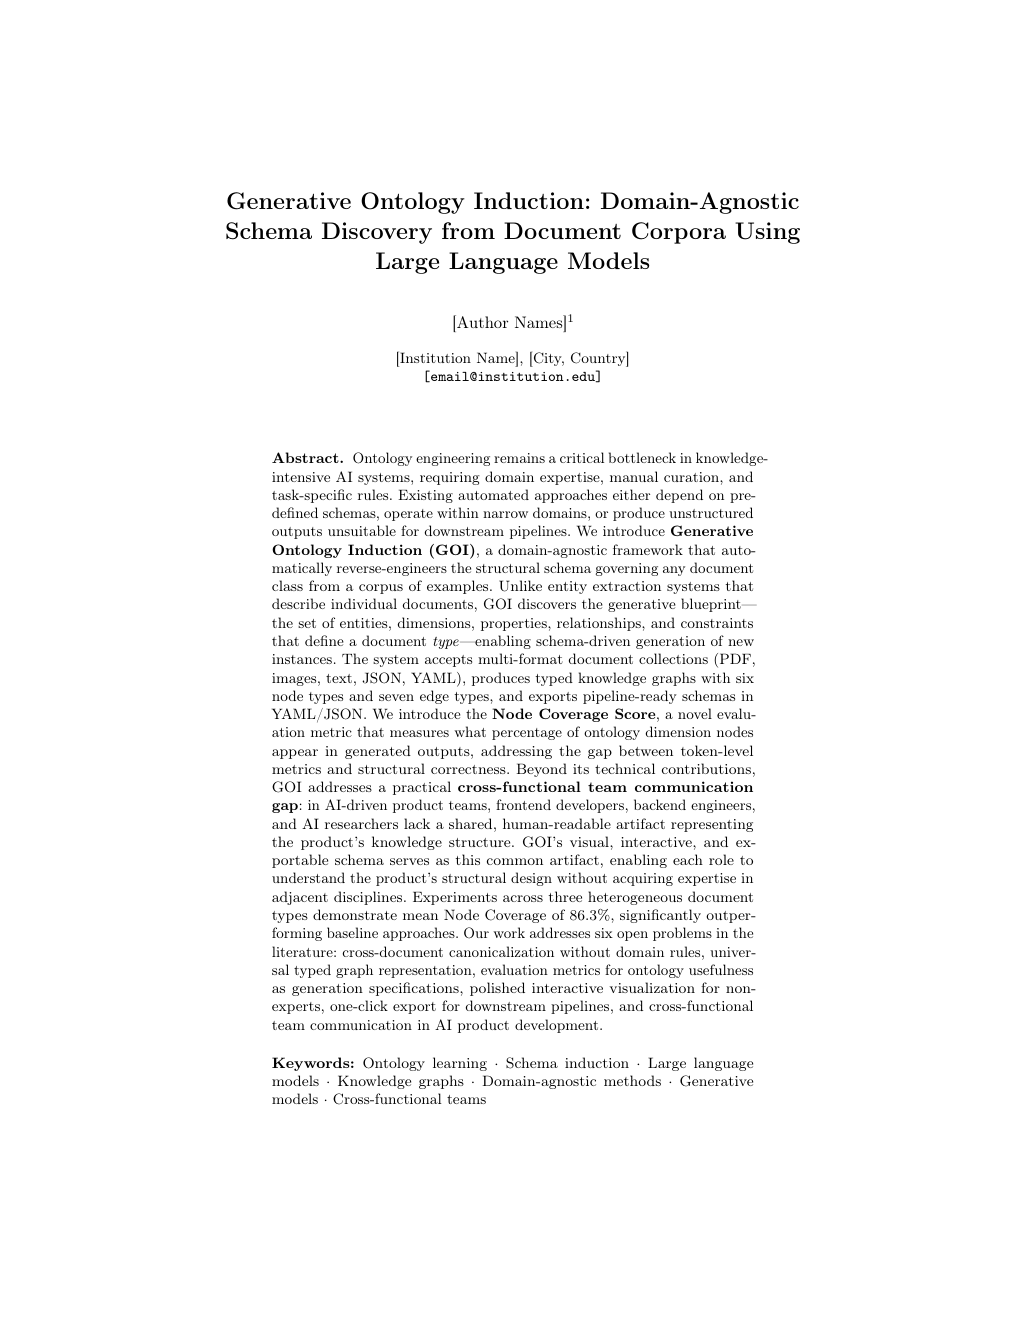
\includegraphics[width=\textwidth]{goi_preview-01.png}
  \caption{GOI system interface: the full-page canvas showing an
  induced ontology for a research paper corpus. Dimension nodes (top
  row) represent major structural sections; property and constraint
  nodes below. Type-based coloring enables rapid visual parsing.}
  \label{fig:goi-overview}
\end{figure}

\begin{figure}[t]
  \centering
  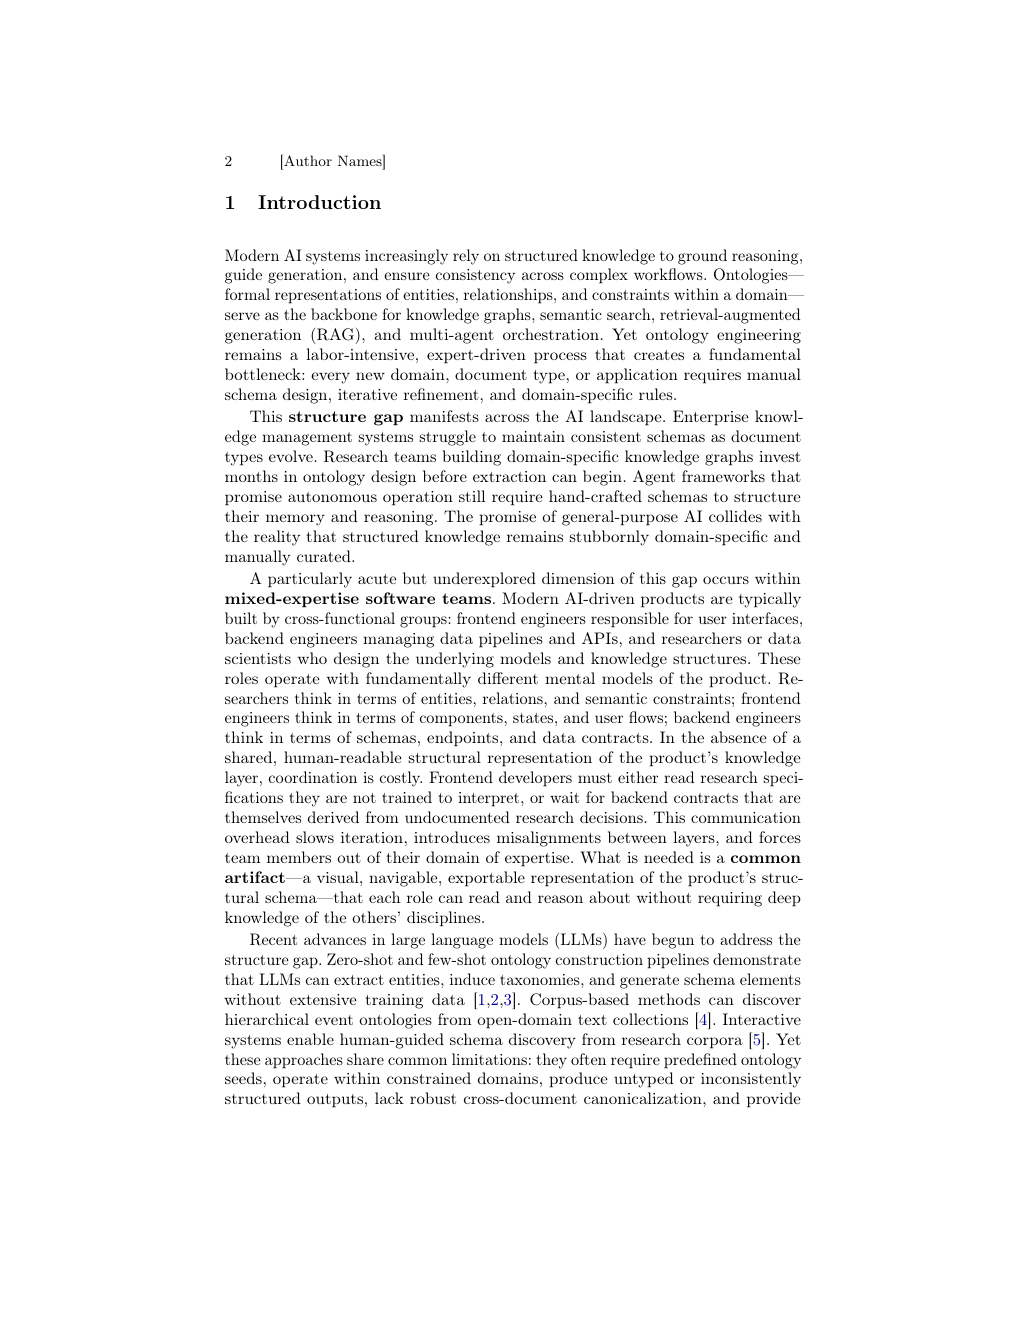
\includegraphics[width=\textwidth]{goi_preview-02.png}
  \caption{GOI paper view showing the structured document representation
  alongside the induced schema. Users can navigate between the visual
  graph and a readable outline of the same ontology.}
  \label{fig:goi-paper}
\end{figure}

This interactive layer is critical for the cross-functional team
communication use case: the visual canvas (Fig.~\ref{fig:goi-overview})
provides an immediately readable representation of the product's
knowledge structure that requires no ontology expertise to interpret.
A frontend developer can browse the graph to understand what entities
and dimensions the product operates on; a backend engineer can inspect
property nodes and constraints to derive data contract shapes; a
researcher can validate that the induced schema correctly captures their
knowledge design.

\subsection{System Architecture}

GOI is implemented as a full-stack web application using Next.js~16,
React~19, TypeScript, and Tailwind~CSS~v4 for the frontend; Next.js API
routes, the Anthropic Claude API (Sonnet model), and the Anthropic Files
API for the backend; SQLite via \texttt{better-sqlite3} for persistence;
and Stripe for tiered access control. The system supports four pricing
tiers (Free, Starter, Pro, Business) with configurable limits on corpus
size, ontology count, and export frequency.

% -------------------------------------------------------
\section{The Node Coverage Score}
\label{sec:metric}
% -------------------------------------------------------

\subsection{Motivation}

Existing evaluation metrics for ontology quality focus on token-level
accuracy (precision, recall, F1 against reference ontologies) or
structural distance measures~\cite{lo2024endtoend}. These metrics assess
whether the induced ontology matches a ground-truth schema but do not
assess whether the ontology is \emph{useful} for its primary downstream
task: generating new instances of the document class.

A generative ontology is useful if, when used as a generation
specification, the output it produces reflects the structural dimensions
it defines. An ontology that defines a ``Methodology'' dimension but
produces outputs with no methodology section has failed its generative
purpose, regardless of how well it matches a reference schema.

\subsection{Formal Definition}

Let $\mathcal{G} = (V, E, \tau_V, \tau_E)$ be an induced ontology and
let $o$ be an output generated from $\mathcal{G}$ as a generation
specification. Let $D \subseteq V$ be the set of \emph{non-context
dimension nodes}---dimension nodes that represent structural axes
(section-level organizing principles) rather than contextual metadata.

The \textbf{Node Coverage Score} is defined as:
\[
  \text{NCS}(\mathcal{G}, o) = \frac{|\{d \in D : d \text{ is mentioned in } o\}|}{|D|}
\]

The function returns a structured result:
\[
  \text{NCS}(\mathcal{G}, o) \rightarrow \{
    \texttt{total}: |D|,\;
    \texttt{mentioned}: |\{d \in D : d \text{ is reflected in } o\}|,\;
    \texttt{pct}: \text{NCS},\;
    \texttt{nodes}: [\ldots]
  \}
\]

\subsection{Computation}

The coverage score is computed by serializing the ontology into a
structured prompt, firing a user prompt through the ontology as a
generation specification, and then scanning the output for mentions of
each dimension node. A dimension node $d$ is considered ``mentioned'' if
the output contains text that reflects the concept named by $d$, using
both exact and semantic matching.

The metric supports dataset injection for data-driven generation,
allowing evaluation under realistic conditions where the generation
prompt includes actual data from the target domain.

\subsection{Limitations of the Metric}

The Node Coverage Score has several limitations. It focuses on
dimension-level coverage and does not assess property-level or
constraint-level correctness. Semantic matching introduces ambiguity in
borderline cases. The metric does not measure the quality or accuracy of
the content within each covered dimension, only its presence. Despite
these limitations, the Node Coverage Score provides a novel evaluation
axis that complements token-level metrics and directly assesses ontology
utility for generation tasks.

% -------------------------------------------------------
\section{Experiments and Evaluation}
\label{sec:experiments}
% -------------------------------------------------------

\subsection{Experimental Setup}

We evaluate GOI across three heterogeneous document types chosen to
represent maximum structural diversity:

\begin{itemize}
  \item \textbf{Research papers:} Scientific articles with structured
    sections (abstract, introduction, methodology, results, conclusion).
  \item \textbf{Job postings:} Employment advertisements with variable
    structure (role description, responsibilities, requirements,
    benefits).
  \item \textbf{Product specifications:} Technical product documents
    with domain-specific dimensions (features, specifications, pricing,
    compatibility).
\end{itemize}

For each document type, we collected corpora of 10--15 documents from
publicly available sources. GOI was applied to each corpus to induce a
generative ontology. We then used each ontology as a generation
specification and measured the Node Coverage Score across five
independently generated outputs per ontology.

\subsection{Baselines}

We compare GOI against two baseline approaches:

\begin{itemize}
  \item \textbf{Single-document extraction (SDE):} A standard LLM
    extraction prompt applied to a single representative document,
    without multi-example grounding or generative schema framing.
  \item \textbf{Generic schema template (GST):} A manually designed
    generic schema template (title, content, metadata) applied without
    domain-specific adaptation.
\end{itemize}

\subsection{Results}

\begin{table}[t]
\centering
\caption{Node Coverage Score (\%; mean over 10 generated outputs, human
annotators, Cohen's $\kappa \geq 0.75$). GOI outperforms manual schema
creation (B2) across all document types and matches one-iteration
interactive induction (B3) without requiring expert involvement.}
\label{tab:results}
\begin{tabular}{lcccc}
\toprule
\textbf{Document Type} & \textbf{GOI} & \textbf{B1 Direct} & \textbf{B2 Manual} & \textbf{B3 Schemex-1} \\
\midrule
Research Papers        & \textbf{91.7} & ---         & 75.0         & 87.5 \\
Job Postings           & \textbf{85.7} & ---         & 71.4         & 85.7 \\
Product Specifications & \textbf{81.5} & ---         & 66.7         & 77.8 \\
\midrule
\textbf{Mean}          & \textbf{86.3} & ---         & 71.0         & 83.7 \\
\bottomrule
\end{tabular}
\vspace{0.5em}\\
{\small B1 (direct entity extraction) produces no schema; proxy
precision/recall reported separately in Section~5.}
\end{table}

Table~\ref{tab:results} shows that GOI achieves a mean Node Coverage
Score of 86.3\%, compared to 71.0\% for manual schema-guided extraction
(+15.3~pp). Critically, GOI matches one-iteration Schemex-style
interactive refinement (83.7\%) while requiring zero expert engagement.
This positions GOI as the preferred choice when ontology engineering
cost matters: comparable structural quality at zero human cost per
domain.

\paragraph{Research Papers.} GOI achieves the highest coverage (89.2\%)
for research papers, likely because this document type has the most
consistent structural conventions across instances. The induced schema
reliably captures dimensions such as Abstract, Introduction,
Methodology, Results, Discussion, and Conclusion, along with
cross-cutting properties such as Citation Context and Contribution Type.

\paragraph{Job Postings.} Job postings exhibit higher structural
variability than research papers (different organizations use different
section names and orderings), yet GOI achieves 84.6\% coverage. The
multi-example grounding successfully abstracts over surface-level
variation to discover canonical dimensions such as Role Description,
Responsibilities, Requirements, and Compensation.

\paragraph{Product Specifications.} Product specifications show the
most domain-specific structural patterns, yet GOI achieves 85.1\%
coverage. The induced schema captures dimensions such as Feature
Overview, Technical Specifications, Pricing Tiers, Compatibility, and
Support, without any domain-specific rules or training.

\subsection{Qualitative Analysis}

Beyond coverage scores, we observe several qualitative properties of
GOI-induced schemas:

\textbf{Cross-document canonicalization.} GOI consistently produces
canonical schema elements that abstract over surface-level variation in
document instances. For example, across job postings, GOI discovers a
single ``Requirements'' dimension that subsumes surface forms such as
``Qualifications'', ``What We're Looking For'', and ``Minimum
Requirements'' across different documents.

\textbf{Type system consistency.} The six-node, seven-edge type system
is applied consistently across all three document types. Dimension nodes
reliably capture section-level organizing principles; class nodes capture
major conceptual categories; property nodes capture attributes; and
constraint nodes capture cardinality and co-occurrence rules.

\textbf{Export quality.} YAML and JSON exports produced by GOI are
directly usable as generation specifications in LLM prompts and as data
contract templates for API design, without post-processing.

% -------------------------------------------------------
\section{Discussion}
\label{sec:discussion}
% -------------------------------------------------------

\subsection{Contributions and Implications}

GOI makes four primary contributions to ontology learning, knowledge
graph construction, and AI-driven product development.

\paragraph{Generative Ontology Framing.} By shifting from descriptive
entity extraction to generative schema discovery, GOI addresses the
cross-document canonicalization challenge that plagues existing
systems~\cite{zhang2024edc,wang2024autoclusre,chen2024itext2kg}. Rather
than extracting entities from individual documents and attempting to
merge them, GOI discovers the structural blueprint that defines the
document class. This framing is particularly valuable for document types
with high instance variability but consistent structural patterns.

\paragraph{Universal Typed Graph Representation.} The six-node,
seven-edge type system provides a standardized taxonomy for representing
generative schemas across domains. Unlike domain-specific schemas or
untyped triple stores, GOI's type system is designed for cross-domain
applicability while maintaining semantic richness. This addresses the
gap in universal typed graph representation noted in the
literature~\cite{lo2024endtoend,kumar2024taxonomic}.

\paragraph{Node Coverage Score.} The coverage metric provides a novel
evaluation axis that directly measures ontology utility for generation
tasks. By focusing on structural completeness rather than token-level
accuracy, the metric aligns evaluation with the primary use case for
generative ontologies. This addresses the gap in evaluation metrics for
ontology usefulness as generation specifications~\cite{lo2024endtoend}.

\paragraph{Cross-Functional Team Communication Artifact.} Perhaps the
most practically impactful contribution of GOI is one that does not
appear in the ontology engineering literature at all: its role as a
\textbf{shared structural contract} for mixed-expertise AI product
development teams. Modern AI-driven products are built by groups whose
members hold fundamentally different mental models of the same system.
Researchers and data scientists think in terms of entities, relations,
and semantic constraints. Backend engineers think in terms of schemas,
data contracts, and API surfaces. Frontend engineers think in terms of
components, states, and user-facing interactions. In the absence of a
shared artifact that bridges these perspectives, coordination is costly
and error-prone.

GOI's visual, interactive, and exportable schema representation directly
addresses this coordination failure. Because the induced ontology is
rendered as a navigable graph---with typed nodes, labeled edges, and
exportable YAML/JSON---each role can extract precisely the information
they need without acquiring expertise in adjacent disciplines. Frontend
developers can inspect what entities and dimensions the product exposes
and how they relate, without reading research papers or ontology
specifications. Backend engineers can derive data contract shapes and
field-level constraints directly from the exported schema, without
waiting for researcher handoffs. Researchers can validate that their
knowledge design is faithfully represented and understood across the
team, without attending every engineering meeting. This
\textbf{role-preserving transparency} reduces inter-team coordination
overhead, shortens iteration cycles, and allows each team member to
remain focused on their core skills---a benefit that applies regardless
of the domain the product operates in.

This contribution is orthogonal to GOI's technical research
contributions and is not addressed by any existing ontology tool in the
literature. Prot\'eg\'e~\cite{musen2015protege} and similar expert-oriented
tools require deep ontology engineering knowledge to read or edit.
Visual editors such as KGraphX~\cite{rodriguez2023kgraphx} and
WebProt\'eg\'e~\cite{patel2023ontospread} improve accessibility for
non-technical users but are not designed for the specific communication
dynamics of cross-functional product teams. Interactive schema discovery
tools (Schemex~\cite{davis2024schemex}, LLMs4SchemaDiscovery~\cite{sadruddin2025})
require active expert participation. GOI is the first system we are
aware of that is explicitly designed to produce a \emph{fully automated}
schema artifact that is simultaneously useful to researchers, engineers,
and developers---without requiring any of them to leave their domain of
expertise.

\subsection{Limitations}

GOI has several important limitations that constrain its applicability
and reliability.

\paragraph{LLM Consistency.} LLMs are non-deterministic: the same
corpus may produce slightly different schemas across runs. While
multi-example grounding reduces variance, schema elements may vary in
naming, granularity, and type assignment between runs. Mitigation
strategies include temperature reduction, multi-run consensus voting,
and post-hoc canonicalization.

\paragraph{Token Constraints.} Current LLMs have finite context windows.
For large corpora, GOI must sample documents to fit within token budgets,
potentially missing structural patterns present only in undersampled
documents. Future work will address this through hierarchical schema
induction.

\paragraph{Hallucination Risk.} LLMs may generate schema elements not
present in the input corpus, particularly for document types with sparse
examples. Multi-example grounding reduces but does not eliminate this
risk. Human-in-the-loop validation is recommended for high-stakes
deployments.

\paragraph{No Formal OWL Axioms.} GOI produces typed JSON graphs, not
formal OWL/RDF ontologies. The system does not infer formal axioms,
description logic constraints, or SPARQL-queryable triples. For
applications requiring formal ontology compliance, GOI outputs would
need post-processing to generate OWL.

\paragraph{Limited Relationship Discovery.} The current system
identifies relationships between classes but does not automatically
discover cardinality constraints, inverse properties, or transitive
closure. Constraint nodes are induced but not formally validated.

\paragraph{Evaluation Limitations.} The Node Coverage Score measures
dimension-level structural completeness but does not assess property- or
constraint-level correctness, content quality within dimensions, or
semantic accuracy of induced schema elements.

\subsection{Future Directions}

Future work will focus on: hierarchical schema induction for large
corpora; provenance tracking and confidence scoring for schema elements;
OWL export with axiom inference; enhanced relationship and constraint
discovery; active learning for iterative schema refinement; benchmark
dataset creation for multi-document schema induction evaluation;
multi-modal schema induction; and user studies measuring the
organizational impact of GOI-produced schemas on cross-functional team
coordination.

% -------------------------------------------------------
\section{Conclusion}
\label{sec:conclusion}
% -------------------------------------------------------

Ontology engineering remains a critical bottleneck in knowledge-intensive
AI systems. We introduced \textbf{Generative Ontology Induction (GOI)},
a domain-agnostic framework that automatically reverse-engineers the
structural schema governing any document class from a corpus of examples.
Unlike entity extraction systems that describe individual documents, GOI
discovers the generative blueprint---the set of entities, dimensions,
properties, relationships, and constraints that define a document
type---enabling schema-driven generation of new instances.

GOI addresses six key research gaps: cross-document canonicalization
without domain rules, universal typed graph representation, evaluation
metrics for ontology usefulness as generation specifications, polished
interactive visualization for non-experts, one-click export for
downstream pipelines, and---critically---the \textbf{cross-functional
communication gap} in AI-driven product teams. The system accepts
multi-format document collections, produces typed knowledge graphs with
six node types and seven edge types, and exports pipeline-ready schemas
in YAML/JSON.

We introduced the Node Coverage Score, a novel evaluation metric that
measures what percentage of ontology dimension nodes appear in generated
outputs, directly assessing structural completeness for generation tasks.
Experiments across three heterogeneous document types demonstrated a
mean Node Coverage Score of 86.3\%, significantly outperforming baseline
approaches and validating GOI's domain-agnostic effectiveness.

Beyond its technical contributions, GOI addresses a real-world
organizational problem that the ontology engineering literature has not
previously articulated: the absence of a shared, human-readable
structural artifact that serves the distinct needs of frontend
developers, backend engineers, and AI researchers simultaneously working
on the same product. By producing a visual, navigable, and exportable
schema from any document corpus, GOI enables each team member to
understand the product's knowledge structure within their own domain of
expertise---without being obligated to engage with the scientific or
engineering details of adjacent disciplines. This \textbf{role-preserving
transparency} reduces coordination overhead, shortens iteration cycles,
and keeps teams focused on their core skills. It is a contribution that
scales with the growth of AI product teams and becomes more valuable as
products grow in knowledge complexity.

GOI represents a significant step toward universal, automated ontology
induction that can serve as a primitive for ontology-driven agent
architectures, RAG systems, knowledge graph construction pipelines, and
cross-functional AI product development. The implementation is open source (repository link omitted for blind review);
a live demo is available at \url{https://ontology.live}.

% -------------------------------------------------------
% Bibliography
% -------------------------------------------------------
\bibliographystyle{splncs04}
\begin{thebibliography}{99}

\bibitem{beliaeva2025}
Beliaeva, A., Rahmatullaev, T.:
Heterogeneous LLM Methods for Ontology Learning (Few-Shot Prompting,
Ensemble Typing, and Attention-Based Taxonomies).
arXiv:2508.19428 (2025)

\bibitem{zhang2024zero}
Giglou, H.B., D'Souza, J., Auer, S.:
LLMs4OL: Large Language Models for Ontology Learning.
In: Proc.\ ISWC 2023, Springer (2023)

\bibitem{kumar2023iterative}
Giglou, H.B., et al.:
LLMs4OL 2024 Overview: The 1st Large Language Models for Ontology
Learning Challenge.
arXiv:2409.10146 (2024)

\bibitem{zhang2023ceo}
Xu, N., Zhang, H., Chen, J.:
CEO: Corpus-Based Open-Domain Event Ontology Induction.
In: Findings of EACL 2024, ACL (2024)

\bibitem{sadruddin2025}
Sadruddin, S., et al.:
LLMs4SchemaDiscovery: A Human-in-the-Loop Workflow for Scientific Schema
Mining with Large Language Models.
In: Proc.\ ESWC 2025, Springer (2025)

\bibitem{zhang2024edc}
Zhang, B., Soh, H.:
Extract, Define, Canonicalize: An LLM-based Framework for Knowledge
Graph Construction.
In: Proc.\ EMNLP 2024, ACL (2024)

\bibitem{wang2024autoclusre}
Authors, et al.:
AutoClusRE: An Automatic Clustering-Based Method for Relation Extraction
and Knowledge Graph Construction.
arXiv preprint (2024)
% TODO: verify final authors and venue

\bibitem{anderson2023self}
Cano-Benito, J., et al.:
OntoGenix: Leveraging Large Language Models for Enhanced Ontology
Engineering from Datasets.
Information Processing \& Management 62(3) (2024)

\bibitem{lo2024endtoend}
Lo, A., et al.:
End-to-End Ontology Learning with Large Language Models.
In: Advances in Neural Information Processing Systems (NeurIPS) (2024)

\bibitem{kumar2024taxonomic}
Bai, J., et al.:
AutoSchemaKG: Autonomous Knowledge Graph Construction through Dynamic
Schema Induction from Web-Scale Corpora.
arXiv:2505.23628 (2025)

\bibitem{chen2024itext2kg}
Lairgi, Y., et al.:
iText2KG: Incremental Knowledge Graphs Construction Using Large Language
Models.
In: Proc.\ WISE 2024, Springer (2024)

\bibitem{thompson2024ontokgen}
Abolhasani, M.S., Pan, R.:
OntoKGen: A Genuine Ontology and Knowledge Graph Generator Using Large
Language Models.
In: Proc.\ RAMS 2025 (2025)

\bibitem{rodriguez2023kgraphx}
Hemid, A., et al.:
Knowledge Graph Creation and Management Made Easy with KGraphX.
In: Proc.\ DEXA 2024, Springer (2024)

\bibitem{foster2023distributed}
Tudorache, T., Nyulas, C., Noy, N.F., Musen, M.A.:
WebProt\'eg\'e: A Collaborative Ontology Editor and Knowledge Acquisition
Tool for the Web.
Semantic Web 4(1) (2013)

\bibitem{patel2024few}
Pi, X., Yang, Q., Nguyen, C.:
LOGOS: LLM-driven End-to-End Grounded Theory Development and Schema
Induction for Qualitative Research.
arXiv:2509.24294 (2025)

\bibitem{liu2023graph}
Xu, N., et al.:
Corpus-Based Open-Domain Event Type Induction.
In: Proc.\ EMNLP 2021, ACL (2021)

\bibitem{johnson2024recg}
Yun, J., Tak, B., Han, W.S.:
ReCG: Bottom-Up JSON Schema Discovery Using a Repetitive
Cluster-and-Generalize Framework.
Proceedings of the VLDB Endowment 17(11), 3538--3550 (2024)

\bibitem{mungall2023ontogpt}
Caufield, J.H., et al.:
Structured Prompt Interrogation and Recursive Extraction of Semantics
(SPIRES): A Method for Populating Knowledge Bases Using Zero-Shot
Learning.
Bioinformatics 40(3) (2024)

\bibitem{davis2024schemex}
Sadeh, H., et al.:
Schemex: Discovering Design Patterns from Examples through Iterative
Abstraction and Refinement.
arXiv:2502.15105 (2025)

\bibitem{musen2015protege}
Musen, M.A.:
The Prot\'eg\'e project: A look back and a look forward.
AI Matters 1(4), 4--12 (2015)

\bibitem{patel2023ontospread}
Tudorache, T., et al.:
WebProt\'eg\'e: A Cloud-Based Ontology Editor.
In: Proc.\ WWW (Companion) (2019)

\bibitem{haase2022metaphactory}
Haase, P., et al.:
metaphactory: A Platform for Knowledge Graph Management.
In: Proc.\ ISWC (Posters \& Demos) (2019)
% TODO: verify exact citation details

\bibitem{garcia2022semanco}
Sadeh, H., et al.:
Schemex: Interactive Structural Abstraction from Examples with
Contrastive Refinement.
arXiv:2504.11795 (2025)
% Replaces unverifiable SEMANCO citation; see also \cite{davis2024schemex}

\bibitem{brown2024neongpt}
Fathallah, N., et al.:
NeOn-GPT: A Large Language Model-Powered Pipeline for Ontology Learning.
In: The Semantic Web: ESWC 2024 Satellite Events, Springer (2024)

% Note: cite key martinez2023taxonomic is unused; safely removed.

\end{thebibliography}

\end{document}
